\section{Appendix}
\label{sec:appendix}

\subsection{Object oriented programming}

There are two main class structures used in the program, one to represent graphs and one to represent different computational methods.

The class \texttt{NodeSet} exists to model a graph. This is done by storing all nodes, each in an instance of the class \texttt{Node}, and their neighbors, where each \texttt{Node} has a list of pointers to all its neighbors. To model sources and sinks, the classes \texttt{Source} and \texttt{Sink} exists, and they are both subclasses of \texttt{Node}. This is in itself enough to model a graph, but there are also some extensions to help dealing with graphs where every node has a given position in a Euclidean space. To do this, the classes \texttt{PositionedNodeSet}, \texttt{PositionedNode}, \texttt{PositionedSource}, and \texttt{PositionedSink} are introduced, which are all similar to their non-positioned versions. These classes are then used as tools when implementing the actual computations.

The class structure allows to implement different computation algorithms using the same framework. To do this, there exists the abstract class \texttt{Algorithm}, which contains a few pure virtual methods that must be implemented by each subclass. The main subclass of \texttt{Algorithm} is \texttt{CurrentWalk}, which implements the current-reinforced random walks. Each instance of \texttt{Algorithm} expects to be given a single \texttt{Node} and uses that as the basis for its calculations.

These two groups of classes are then used by the main program to perform simulations. Given a method to create instances of some subclass of \texttt{Algorithm}, the main program is then able to construct a \texttt{NodeSet} with a set of \texttt{Node}s and an \texttt{Algorithm} for each \texttt{Node}. The algorithm advances using the \texttt{takeStep()} method in \texttt{NodeSet}. A schematic overview of this structure is shown in Figure. (\ref{fig:graphToClass}).

\begin{figure}[H]
\centering
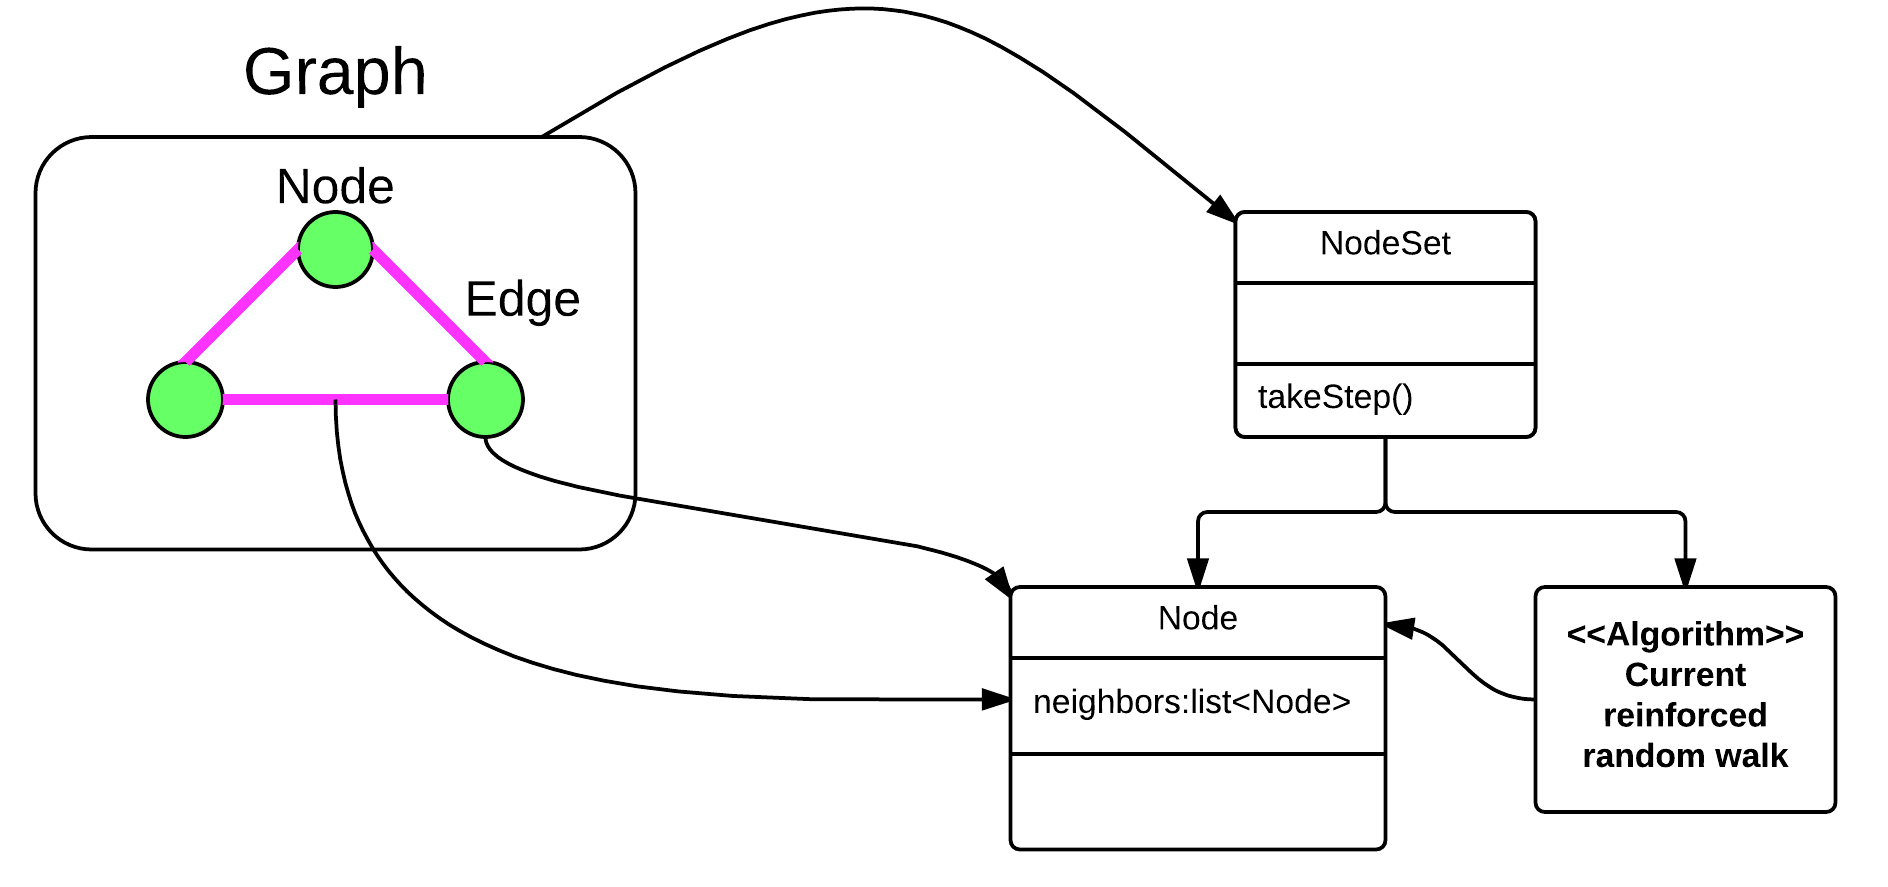
\includegraphics[width=0.95\textwidth]{img/graphToClass.png}
\caption{An overview of the relation between elements in the graph and different classes in the program structure. It can be seen that each \texttt{NodeSet} contains both a set of \texttt{Node}s and a set of \texttt{Algorithm}s.}
\label{fig:graphToClass}
\end{figure}

\subsection{Metis and parallelism}

%\subsection{Algorithm}
%\label{sec:appendix:algorithm}
%The probability for a particle to move to another node in this particular current-reinforced random walk depends on the flow of particles to that node, i.e. the current of particles. This optimizes the path length for each individual path from the sources to the sinks, i.e it minimizes 
%
%\begin{equation}
%\sum_{j \in \text{Neighbors}(i)} l_{ij} \bar{I}_{ij},
%\end{equation}
%
%\noindent where $l_{ij}$ is the edge length between node $i$ and $j$ and $\bar{I}_{ij}$ is the corresponding mean flow of particles. When utilizing non linear current-reinforced random walks a combination of path length and path maintenance is optimized. 
%
%There are some necessary parameters for this model to make sense. These parameters and their analogy in both electrical networks and ant trail networks are shown in Table \ref{tab:parameters}.
%
%\begin{table}
%\centering
%\caption{Table shows the necessary parameters for the current-reinforced random walk modeling and their analogy in electrical networks and ant trail networks. $i$ denotes that the parameter corresponds to node $i$ and $ij$ denotes that the parameter corresponds to the edge between node $i$ and node $j$.}
%\label{tab:parameters}
%\begin{tabular}{ c | c | c }                       
%	\textbf{Parameter} & \textbf{Electrical network} & \textbf{Ant trails} \\
%	\hline
%	$l_{ij}$ & length in space & length in space \\
%	\hline
%	$N_{i}$ & number of electrons & number of ants \\
%	\hline	
%	$P_{i}$ & potential & inverse flowness \\
%	\hline
%	$I_{ij}$ & current & flow of ants \\
%	\hline
%	$D_{ij}$ & conductivity & pheromone concentration \\
%	\hline
%	$C_{i}$ & capacitance & total pheromone density \\
%	\hline
%	$q$ & reinforcement intensity & pheromone drop rate \\
%	\hline
%	$\lambda$ & conductivity decrease rate & pheromone evaporation rate \\
%\end{tabular} 
%\end{table}
%
%\subsubsection{Preparation}
%The preparation begins with each node calculating the mean flow to each of its neighbors as
%\begin{equation}
%\bar{I}_{ij} = \frac{(N_i - N_j)D_{ij}}{l_{ij}},
%\end{equation}
%from which it can be seen that the mean flow depends on the conductivity of each edge, $D_{ij}$, which is 	initialized at and kept at or above some minimal value.
%The actual flow along the edge $ij$ can then be found as
%\begin{equation}
%I_{ij} = \text{Poi}(|\bar{I}_{ij}|\Delta t).
%\end{equation}
%In terms of implementation, it is important that nodes that are connected to the same edge agree on the same number of particles to transfer. This is ensured by allowing only the node with a larger number of particles to randomize the value and then both nodes use that value when updating the number of particles. This work is done at the node with the largest number of particles, since it is also important to ensure that there are never fewer than zero particles at a node and the number of particles will be decreasing at the node with the largest number of particles. When a node has a smaller number of particles than a given neighbor, the node always calculates the flow to that neighbor as zero. After all nodes have calculated and stored $\bar{I}$ and $I$, the preparation step is finished.
%
%\subsubsection{Confirmation}
%At the beginning of the confirmation part, all the data regarding how many particles will move along each edge is available. And so each node begins by updating the number of particles that is has as
% \begin{equation}
% N_i(t + \Delta t) = N_i(t) + \sum_{j \in \text{Neighbors}(i)} \left( I_{ji} - I_{ij} \right)
% \end{equation}
% The flow should theoretically be symmetric, but since only one particle has randomized a value, and the other has set it to zero, the flow is not symmetric in this implementation.
% 
%After that, the final part of the step begins, in which several parameters that are relevant to the algorithm are updated. First is the conductivity, which can be calculated as
%\begin{equation}
%D_{ij}(t + \Delta t) = D_{ij}(t) + q|\bar{I}|^\mu - \lambda D_{ij}(t)\Delta t,
%\end{equation}
%
%where $q$ is the reinforcement intensity caused by per unit flow, $\mu$ is the path maintenance parameter, $\lambda$ is the conductivity decay parameter and $\Delta t$ is the time step. If $\mu$ is set to one the current-reinforced random walk is linear and will converge to the same solution every time. If on the other hand $\mu$ is set to greater than one the current-reinforced random walk becomes non-linear and will not converge to the same solution every time that a system is simulated. 
%
%Next to be calculated is the capacitance, which is calculated as 
% \begin{equation}
% C_i = \sum_{j \in \text{Neighbors}(i)} D_{ij}
% \end{equation}
% and finally the potential is calculated as
% \begin{equation}
% P_i = \frac{N_i}{C_i}.
% \end{equation}
% 
% \noindent When this is done the step is finished and the next step can be started.